\documentclass[twoside,letterpaper,10pt]{article}

\usepackage{mystyle}
% TODO make the background of theorems darker (or at least make sure that the
% printer does).
\usepackage{wrapfig}
\newcommand{\KAM}{ Let $\rho, \gamma > 0$ be given, and let
  $h(\bp{q}, \bp{p}) = h_0(\bp{p}) + h_1(\bp{q}, \bp{p})$ be a Hamiltonian, with
  $h_0, h_1 \in \mathcal{A}_{\rho}$ and $\norm{h}_{\rho} \leq 1$.
  Suppose the Taylor polynomial of $h_0$ is
  \begin{equation*}
    h_0(\bp{p}) = a + \omega\bp{p} + \frac{1}{2} \bp{p} \cdot C \bp{p} +
    o(|\bp{p}|^2),
  \end{equation*}
  with $\omega \in \Omega_{\gamma}$ and $C$ is symmetric and invertible.
  Then for any $\rho_* \leq \rho$, there exists $\epsilon > 0$, which depends on
  $C$ and $\gamma$, but not on the remainder term in $o(|\bp{p}|^2)$, such that
  if $\norm{h_1}_{\rho} \leq \epsilon$, there exists a symplectic mapping $\Phi
  : A_{\rho_*} \to A_{\rho}$ such that if we set $(\bp{q}, \bp{p}) = \Phi(\bp{Q},
  \bp{P})$ and $H = h \circ \Phi$, we have
  \begin{equation*}
    H(\bp{Q}, \bp{P}) = A + \omega \bp{P} + R(\bp{Q}, \bp{P}),
  \end{equation*}
  with $R(\bp{Q}, \bp{P}) \in O(|\bp{P}|^2)$.
}

\newcommand{\dionumber}{
  A number $\theta$ is \emph{Diophantine of exponent d} if there exists a
    constant $\gamma > 0$ such that for all coprime integers $p$ and $q$ we have
    \begin{equation*}
      \left| \theta - \frac{p}{q} \right| > \frac{\gamma}{|q|^d}.
    \end{equation*}
}

\newcommand{\diovector}{
  Let $\omega = (\omega_1, \ldots, \omega_n)$.
    We say $\omega$ is Diophantine if there exists $\gamma > 0$ such that for
    all vectors with integer coefficients $(k_1, \ldots, k_n)$, we have
    \begin{equation*}
      |k_1 \omega_1 + \cdots + k_n \omega_n| \geq \frac{\gamma}{(k_1^2 + \cdots
        + k_n^2)^{\frac{n}{2}}}.
    \end{equation*}
    Let $\Omega_{\gamma}^n$ be the subset of such $\omega \in \R^n$.
}

\newcommand{\domains}{
  \begin{align*}
    B_{\rho} &= \{\bp{p} \in \C : |\bp{p}| \leq \rho\},\\
    C_{\rho} &= \{\bp{q} \in \C^n / \Z^n : | \Imag(\bp{q}) | \leq \rho\},\\
    A_{\rho} &= C_{\rho} \times B_{\rho} = \{(\bp{q}, \bp{p}) \in \C^n / \Z^n
               \times \C^n : |\bp{p}| \leq \rho, \, |\Imag(\bp{q})| \leq \rho\}.
  \end{align*}
}



\title{The Kolmogorov Theorem}
\author{Travis Westura}
\date{\today}

\begin{document}

\maketitle

% I know that I'm not supposed to use a citation in an abstract, but Hubbard
% did so in his paper, so I guess it is fair game.
\begin{abstract}
  This paper gives a proof of the Kolmogorov Theorem on the conservation of
  invariant tori.
  We follow the approach given by Hubbard and Ilyashenko in .
  Their proof is similar to the one given by Bennettin, Galgani, Giorgilli, and
  Strelcyn in , which itself resembles Kolmogorov's original argument.
  % TODO write citations and confirm correctness of the last claim by rereading
  % the other paper's abstract.
  % Also check the spelling of their names and add them to the dictionary.
  % Do by 4/27.
\end{abstract}


\section{Introduction}
\label{sec:introduction}

% TODO Write up historical information in the next paragraph.

But before moving on, let's take a look at our main goal:
\begin{thm}[The Kolmogorov Theorem]
  \label{thm:KAM}
  \KAM{}
\end{thm}
We will return to this statement after building up some intuition for it.

\section{A Motivating Example}
\label{sec:motivating-example}

To start understanding the theorem, let's consider an example to which we would
like to apply it.
While staring up at the night sky, one might be driven to wonder, ``Why do the
planets orbit around the sun and just not fly off by themselves in their own
directions?''


\section{Hamiltonian Mechanics}
\label{sec:hamilt-mech}



\section{Irrationality}
\label{sec:irrationality}

In our statement of Kolmogorov's Theorem, we included the hypothesis that
$\omega \in \Omega_{\gamma}$.
We now define this notation and begin to explain its importance.
The set $\Omega_{\gamma}$ consists of vectors that are ``sufficiently
irrational,'' a notion that we need to make more precise.

Let's first consider the definition of an irrational number.
If a real number $\theta$ is irrational, then for all pairs if integers $p$ and
$q$, with $q$ positive, we have the following
\begin{equation*}
  \left| \theta - \frac{p}{q} \right| \neq 0.
\end{equation*}
This equation tells us simply that there does not exist and rational number
$\frac{p}{q}$ that equals our irrational number $\theta$.
Here, the ``not equal to zero'' part of the equation will be stressed, as an
expression similar to the one on the left hand side will later appear as the
denominator of a fraction (see \cref{sec:dioph-diff-equat}).
As dividing by zero can be rather troublesome, we wish to avoid it.
This condition of irrationality is the tool we use to do so: if $\theta$ is
irrational, then the left side will not be zero, so we can divide by it without
any problems.

Our condition of ``sufficiently irrational'' will mean that $\left| \theta -
  \frac{p}{q} \right|$ is ``sufficiently nonzero,'' or since we are using an
absolute value, ``sufficiently big.''
However, as we learn in our introductory courses in real analysis, the rationals
are dense in the reals, and every real number, specifically every irrational
number $\theta$, may be approximated arbitrarily closely by the rationals.
More precisely, given any real $\epsilon > 0$, there exists a rational number
$\frac{p}{q}$ such that $\left| \theta - \frac{p}{q} \right| < \epsilon$.
Thus trying to coerce $\left| \theta - \frac{p}{q} \right|$ to be big is quite
impossible.

Unsatisfied with our answer, let's instead consider a different question.
Instead of wanting $\left| \theta - \frac{p}{q} \right|$ to be ``big,'', we ask
that it is small \emph{only if the denominator is big}.
This is the beginning of the theory of Diophantine approximation.

The numbers that we seek will satisfy the following definition.
\begin{defn}[Diophantine Number of Exponent $d$]
  \dionumber{}
\end{defn}
From this definition we see that it is a stronger requirement for a number to be
Diophantine of a smaller exponent.
For all irrational numbers $\theta$ there exist arbitrarily large $q$ and $p$
prime to $q$ such that
\begin{equation*}
  \left| \theta - \frac{p}{q} \right| < \frac{1}{\sqrt{5}q^2}.
\end{equation*}
We see that no number is Diophantine of any exponent smaller than $2$.
And the number that are Diophantine of exponent exactly $2$ are precisely the
numbers whose continued fractions have bounded entries.
These numbers form a set of measure zero.

But what about exponents greater than $2$, or rather, of the form $2 + \epsilon$
for $\epsilon > 0$?
In the sense of Lebesgue measure, these numbers are quite abundant, as for any
$\epsilon > 0$ they form a set of full measure.
\begin{prop}[Diophantine Numbers with Full Measure]
  For all $\epsilon > 0$, the set of Diophantine numbers of exponent $2 +
  \epsilon$ is of full measure.
\end{prop}
\begin{proof}
  % TODO write proof by 4/27.
  We consider numbers in $\R / \Z$.
  Given any positive integer $q$, there are at most $q$ elements of $\Q / \Z$
  that, in reduced form, have denominator $q$.
  Hence for any constant $\gamma$, we consider the set
  \begin{equation*}
    \left\{ \theta \in \R / \Z : \left| \theta - \frac{p}{q} \right| <
      \frac{\gamma}{|q|^{2 + \epsilon}} \right\}.
  \end{equation*}
  The length of this set is at most $\frac{2\gamma}{q^{1 + \epsilon}}$.
  Summing over all $q$, we see that the set of numbers $\theta$ for with there
  exists $q$ such that
  \begin{equation*}
    \left| \theta - \frac{p}{q} \right| < \frac{\gamma}{2^{2 + \epsilon}}
  \end{equation*}
  has length strictly less than
  \begin{equation*}
    2 \gamma \sum_{q = 1}^{\infty} \frac{1}{q^{1 + \epsilon}}.
  \end{equation*}
  Then we take the intersection over all these sets as $\gamma \to 0$, and we
  note that this intersection has measure $0$.
  But this set is the complement of the set of Diophantine numbers of exponent
  $2 + \epsilon$.
  Hence the claim holds.
\end{proof}

% TODO discuss vectors

\section{Analytic Functions}
\label{sec:analytic-functions}

As this is a paper for a complex analysis class, we begin this section by noting
that the complex analysis is located here.

Consider the function $f(x) = x^3 - x + \frac{\sqrt{2}}{2}$.
\begin{wrapfigure}{o}{0.5\textwidth}
  \begin{center}
    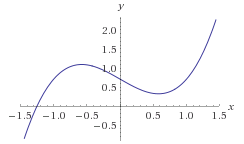
\includegraphics[width=0.48\textwidth]{newtonfail}
  \end{center}
  \caption{$f(x) = x^3 - x + \frac{\sqrt{2}}{2}$}
\end{wrapfigure}

\section{Main Idea of the Proof}
\label{sec:main-idea-proof}

\section{Diophantine Differential Equations}
\label{sec:dioph-diff-equat}

\section{Solving Equations}
\label{sec:solving-equations}



\end{document}

%%% Local Variables:
%%% mode: latex
%%% TeX-master: t
%%% End:
